\begin{flushright} {\tiny {\color{gray} mappings.tex}} \end{flushright}
%~~~~~~~~~~~~~~~~~~~~~~~~~~~~~~~~~~~~~~~~~~~~~~~~~~~~~~~~~~~~~~~~~~~~~~~~~~~~~~~~~~~~~~~~~~~~~~~~~~

\index{general}{Isoparametric}
\index{general}{Subparametric} 
\index{general}{Superparametric}

The name {\sl isoparametric} derives from the fact that the same ('iso') 
functions are used as basis functions and for the mapping to the reference element.

More generally, if $n_e$ denotes the number of nodes of an element and $n_g$ denotes the 
number of nodes describing the geometry of the element, 
then the element is termed {\sl subparametric} when $n_g<n_e$ and 
{\sl superparametric} when $n_g>n_e$.

%...........................................
\subsection{General case}

What follows is written for the 2d case but extending it to 3d is trivial.

Any variable defined on the element can be approximated using the basis functions:
\begin{equation}
f^h(r,s)=\sum_i \bN_i(r,s) f_i.
\end{equation}
If we treat the coordinate variables $x$ and $y$ themselves as functions, 
then the basis functions can be used to construct the mapping:
\begin{eqnarray}
x &=& \sum_{i=1}^4 \bN_i(r,s) x_i \\
y &=& \sum_{i=1}^4 \bN_i(r,s) y_i 
\end{eqnarray}
This is a relationship between the reduced coordinates $r,s$ and the 'real'
coordinates $x,y$.

Let us compute the space derivatives of these quantities:
\begin{eqnarray}
\frac{\partial x}{\partial r} &=& \sum_i \frac{\partial \bN_i}{\partial r} x_i \\
\frac{\partial x}{\partial s} &=& \sum_i \frac{\partial \bN_i}{\partial s} x_i \\
\frac{\partial y}{\partial r} &=& \sum_i \frac{\partial \bN_i}{\partial r} y_i \\
\frac{\partial y}{\partial s} &=& \sum_i \frac{\partial \bN_i}{\partial s} y_i 
\end{eqnarray}

We also have 
\begin{eqnarray}
\frac{\partial f}{\partial r} &=&
\frac{\partial f}{\partial x}\frac{\partial x}{\partial r}
+\frac{\partial f}{\partial y}\frac{\partial y}{\partial r} \\
\frac{\partial f}{\partial s} &=&
\frac{\partial f}{\partial x}\frac{\partial x}{\partial s}
+\frac{\partial f}{\partial y}\frac{\partial y}{\partial s}
\end{eqnarray}
or in matrix form:
\begin{equation}
\left(
\begin{array}{c}
\frac{\partial f}{\partial r} \\ \\
\frac{\partial f}{\partial s}
\end{array}
\right)
=
\underbrace{
\left(
\begin{array}{cc}
\frac{\partial x}{\partial r} & \frac{\partial y}{\partial r} \nonumber\\ \\
\frac{\partial x}{\partial s} & \frac{\partial y}{\partial s} \nonumber
\end{array}
\right)
}_{\bm J}
\cdot
\left(
\begin{array}{c}
\frac{\partial f}{\partial x} \\ \\
\frac{\partial f}{\partial y}
\end{array}
\right)
\end{equation}
where ${\bm J}$ is called the Jacobian of the transformation
By inverting the Jacobian matrix, the desired derivatives with respect to $x$
and $y$ can be obtained:
\[
\left(
\begin{array}{c}
\frac{\partial f}{\partial x} \\ \\
\frac{\partial f}{\partial y}
\end{array}
\right)
=
{\bm J}^{-1} \cdot 
\left(
\begin{array}{c}
\frac{\partial f}{\partial r} \\ \\
\frac{\partial f}{\partial s}
\end{array}
\right)
\]
The inverse of the Jacobian matrix can be simply obtained in 
2D (Cramer's rule for $2\times2$ matrices\footnote{\url{https://en.wikipedia.org/wiki/Cramers_rule}}):
\[
{\bm J}^{-1} = \frac{1}{|{\bm J}|} 
\left(
\begin{array}{cc}
\frac{\partial y}{\partial s} & -\frac{\partial y}{\partial r} \nonumber\\ \\
-\frac{\partial x}{\partial s} & \frac{\partial x}{\partial r} \nonumber
\end{array}
\right)
\]
The presence of the determinant in the denominator implies that it cannot 
be zero anywhere, or in other words: the mapping is not valid if $|{\bm J}|$
is zero anywhere over the element.


\begin{remark}
Problems also arise when the Jacobian matrix is nearly singular due to round-off errors.
To avoid problems linked to badly shaped elements, it is recommended that the inside
angles of an element are larger than $15\degree$ and less than $165\degree$.
\end{remark}

From Eq.~\eqref{eqxy}, we can also write:
\begin{eqnarray}
dx &=& \frac{\partial x}{\partial r} dr + \frac{\partial x}{\partial s} ds \\
dy &=& \frac{\partial y}{\partial r} dr + \frac{\partial y}{\partial s} ds 
\end{eqnarray}
or, 
\begin{equation}
\left(
\begin{array}{c}
dx \\ dy
\end{array}
\right)
={\bm J}\cdot
\left(
\begin{array}{c}
dr \\ ds
\end{array}
\right)
\end{equation}
This means that integrating over the 'real' element in $(x,y)$ space
can be simply done by integrating of the reference element in the 
$(r,s)$ space. This is the cornerstone of most of the implementation of the 
Finite Element Method, the second integral being carried out by means 
of the Gauss-Legendre quadrature.

\begin{equation}
\iint_{\Omega_e} ... \; dx dy = \int_{-1}^{+1} \int_{-1}^{+1} ...|{\bm J}| \; dr ds
\end{equation}










%...........................................
\subsection{Linear mapping on a triangle}



\begin{eqnarray}
x 
&=& \sum_{i=1}^3 N_i(r,s) x_i \nonumber\\
&=& N_1(r,s) x_1 +N_2(r,s) x_2 +N_3(r,s) x_3   \nonumber\\
&=&  (1-r-s) x_1 +(r) x_2  +(s) x_3   \nonumber\\
&=& x_1 + (x_2-x_1) r + (x_3-x_1)s \nonumber\\
&=& a_x + b_x r + c_x s \nonumber\\
y 
&=& \sum_{i=1}^3 N_i(r,s) y_i \nonumber\\
&=& N_1(r,s) y_1 +N_2(r,s) y_2 +N_3(r,s) y_3   \nonumber\\
&=&  (1-r-s) y_1 +(r) y_2  +(s) y_3   \nonumber\\
&=& y_1 + (y_2-y_1) r + (y_3-y_1)s \nonumber\\
&=& a_y+ b_y r + c_y s 
\nonumber
\end{eqnarray}

Let us compute the space derivatives of these quantities:
\begin{eqnarray}
\frac{\partial x}{\partial r} &=& x_2-x_1=b_x \nonumber\\
\frac{\partial x}{\partial s} &=& x_3-x_1=c_x \nonumber\\
\frac{\partial y}{\partial r} &=& y_2-y_1=b_y \nonumber\\
\frac{\partial y}{\partial s} &=& y_3-y_1=c_y \nonumber
\end{eqnarray}
The jacobian matrix is then given by
\[
{\bm J} = \left(
\begin{array}{cc}
x_2-x_1 & y_2-y_1 \\
x_3-x_1 & y_3-y_1
\end{array}
\right)
= \left(
\begin{array}{cc}
b_x & b_y \\
c_x & c_y
\end{array}
\right)
\]
and its inverse
\[
{\bm J}^{-1} 
= \frac{1}{b_xc_y-c_xb_y}
\left(
\begin{array}{cc}
c_y& -b_y \\
-c_x & b_x
\end{array}
\right)
=
\frac{1}{2A}
\left(
\begin{array}{cc}
c_y& -b_y \\
-c_x & b_x
\end{array}
\right)
\]
where $A=(b_xc_y-c_xb_y)/2$ is actually the area of the triangle!


The Cartesian basis function derivatives are then
\[
\left(
\begin{array}{c}
\frac{\partial N_1}{\partial x} \\ \\
\frac{\partial N_1}{\partial y}
\end{array}
\right)
=
{\bm J}^{-1}
\cdot
\left(
\begin{array}{c}
\frac{\partial N_1}{\partial r} \\ \\
\frac{\partial N_1}{\partial s}
\end{array}
\right)
=
\frac{1}{2A}
\left(
\begin{array}{cc}
c_y& -b_y \\
-c_x & b_x
\end{array}
\right)
\cdot
\left(
\begin{array}{c}
-1 \\ \\ -1 
\end{array}
\right)
=
\frac{1}{2A} 
\left(
\begin{array}{c}
b_y - c_y \\ 
c_x - b_x
\end{array}
\right)
\]


\[
\left(
\begin{array}{c}
\frac{\partial N_2}{\partial x} \\ \\
\frac{\partial N_2}{\partial y}
\end{array}
\right)
=
{\bm J}^{-1}
\cdot
\left(
\begin{array}{c}
\frac{\partial N_2}{\partial r} \\ \\
\frac{\partial N_2}{\partial s}
\end{array}
\right)
=
\frac{1}{2A}
\left(
\begin{array}{cc}
c_y& -b_y \\
-c_x & b_x
\end{array}
\right)
\cdot
\left(
\begin{array}{c}
1 \\ 0
\end{array}
\right)
=
\frac{1}{2A} 
\left(
\begin{array}{c}
c_y \\ -c_x
\end{array}
\right)
\]



\[
\left(
\begin{array}{c}
\frac{\partial N_3}{\partial x} \\ \\
\frac{\partial N_3}{\partial y}
\end{array}
\right)
=
{\bm J}^{-1}
\cdot
\left(
\begin{array}{c}
\frac{\partial N_3}{\partial r} \\ \\
\frac{\partial N_3}{\partial s}
\end{array}
\right)
=
\frac{1}{2A}
\left(
\begin{array}{cc}
c_y& -b_y \\
-c_x & b_x
\end{array}
\right)
\cdot
\left(
\begin{array}{c}
0 \\ 1 
\end{array}
\right)
=
\frac{1}{2A} 
\left(
\begin{array}{c}
-b_y \\  b_x
\end{array}
\right)
\]











%................................................
\subsection{Bilinear mapping ($Q_1$) on a quadrilateral}

The \index{general}{reference element} reference element 
is in the $(r,s)$ space. It is a square of size $2\times2$ 
centered around the origin, i.e. $(r,s)\in[-1,1]\times[-1,1]$. 
We wish to map it to the quadrilateral in the $(x,y)$ space 
(and vice versa):

\begin{center}
\includegraphics[width=8cm]{images/mappings/bilinear/mapping_bilinear.png}
\end{center}

The coordinates of the vertices are 
$(x_1,y_1)$, $(x_2,y_2)$, $(x_3,y_3)$ and $(x_4,y_4)$.
We then simply have the 
following relationship, i.e. any point of the reference element 
can be mapped to the physical quadrilateral as follows:
\begin{eqnarray}
x&=& \bN_1(r,s) x_1 + \bN_2(r,s) x_2 + \bN_3(r,s) x_3 + \bN_4(r,s) x_4 \\
y&=& \bN_1(r,s) y_1 + \bN_2(r,s) y_2 + \bN_3(r,s) y_3 + \bN_4(r,s) y_4 \label{mapppQ1a} 
\end{eqnarray} 
where the $Q_1$ basis functions $\bN_i(r,s)$ are defined in Section~\ref{sec:elts1D}.

In the following example the program randomly generates 10000 points 
inside the reference 
element and computes their mapping into the $(x,y)$ space. 

\begin{lstlisting}
x1=-1 ; y1=-2
x2=3  ; y2=-1
x3=2  ; y3=2
x4=-3 ; y4=1

npts=10000
r=np.zeros(npts,dtype=np.float64)   
s=np.zeros(npts,dtype=np.float64)   
x=np.zeros(npts,dtype=np.float64)   
y=np.zeros(npts,dtype=np.float64)   

for i in range(0,npts):
    # compute random r,s coordinates
    r[i]=random.uniform(-1.,+1)
    s[i]=random.uniform(-1.,+1)
    # compute basis function values at r,s
    N1=0.25*(1-r[i])*(1-s[i])
    N2=0.25*(1+r[i])*(1-s[i])
    N3=0.25*(1+r[i])*(1+s[i])
    N4=0.25*(1-r[i])*(1+s[i])
    # compute x,y coordinates
    x[i]=N1*x1+N2*x2+N3*x3+N4*x4
    y[i]=N1*y1+N2*y2+N3*y3+N4*y4

np.savetxt('rs.ascii',np.array([r,s]).T)
np.savetxt('xy.ascii',np.array([x,y]).T)
\end{lstlisting}

\begin{center}
\includegraphics[width=7cm]{images/mappings/bilinear/rs.pdf}
\includegraphics[width=7cm]{images/mappings/bilinear/xy.pdf}
\end{center}

There is also an inverse map, which is not so easily computed (see Section~\ref{sec:amiin}).
However, if the quadrilateral in the $(x,y)$ space is a rectangle of size $(h_x,h_y)$, 
the inverse mapping is trivial:
\begin{eqnarray}
r&=&\frac{x-x_1}{x_2-x_1} \\
s&=&\frac{y-y_1}{y_4-y_1} 
\end{eqnarray}
Also in the case of rectangular elements of size $(h_x,h_y)$
the basis functions can easily be written as functions of $(x,y)$:
\begin{eqnarray}
\bN_1(x,y) &=& \left( \frac{x_3 -x }{h_x}  \right) \left( \frac{y_3 -y }{h_y}  \right) \nn\\
\bN_2(x,y) &=& \left( \frac{x - x_1}{h_x}  \right) \left( \frac{y_3 -y }{h_y}  \right) \nn\\
\bN_3(x,y) &=& \left( \frac{x - x_1}{h_x}  \right) \left( \frac{y - y_1}{h_y}  \right) \nn\\
\bN_4(x,y) &=& \left( \frac{x_3 -x }{h_x}  \right) \left( \frac{y - y_1}{h_y}  \right) \nn 
\end{eqnarray}

From Eq.~\eqref{mapppQ1a} and using the expressions for the $Q_1$ basis functions, we can write 
\begin{eqnarray}
x &=& 
 \frac14(x_1+ x_2+ x_3 +x_4) 
+\frac14(-x_1 +x_2 +x_3 -x_4) r 
+\frac14(-x_1 -x_2 +x_3 +x_4) s
+\frac14(x_1 -x_2 +x_3 -x_4) rs \nonumber\\
y &=& 
 \frac14(y_1+ y_2+ y_3 +y_4) 
+\frac14(-y_1 +y_2 +y_3 -y_4) r 
+\frac14(-y_1 -y_2 +y_3 +y_4) s
+\frac14(y_1 -y_2 +y_3 -y_4) rs \nonumber
\end{eqnarray}

Let us compute the space derivatives of these quantities:
\begin{eqnarray}
\frac{\partial x}{\partial r} &=& \frac14(-x_1 +x_2 +x_3 -x_4) +\frac14(x_1 -x_2 +x_3 -x_4) s = A_1 + A_2s\nonumber\\
\frac{\partial x}{\partial s} &=& \frac14(-x_1 -x_2 +x_3 +x_4) +\frac14(x_1 -x_2 +x_3 -x_4) r = A_3 + A_4r\nonumber\\
\frac{\partial y}{\partial r} &=& \frac14(-y_1 +y_2 +y_3 -y_4) +\frac14(y_1 -y_2 +y_3 -y_4) s = B_1 + B_2s\nonumber\\
\frac{\partial y}{\partial s} &=& \frac14(-y_1 -y_2 +y_3 +y_4) +\frac14(y_1 -y_2 +y_3 -y_4) r = B_3 + B_4r \nonumber
\end{eqnarray}



The jacobian matrix is then given by
\[
{\bm J} = \left(
\begin{array}{cc}
A_1 + A_2s & B_1 + B_2s \\
A_3 + A_4r & B_3 + B_4r
\end{array}
\right)
\]
and its inverse
\[
{\bm J}^{-1} = \frac{1}{C}
\left(
\begin{array}{cc}
B_3 + B_4r & -B_1 - B_2s \\
-A_3 - A_4r & A_1 + A_2s
\end{array}
\right)
\]
with $C$ being the determinant given by
\[
C= (A_1 + A_2s)(B_3 + B_4r)-(A_3 + A_4r)(B_1 + B_2s)
\]


%---------------------------------
\subsubsection{A concrete example}

Let us look at this by means of a simple example and let us consider the following 
element:
\begin{center}
\includegraphics[width=4cm]{images/mappings/fournode/ex1}
\end{center}
Then a $Q_1$ mapping yields:
\begin{eqnarray}
x(r,s) &=& \sum_i \bN_i(r,s) x_i = \bN_2 + 2\bN_3 = \frac{1}{4} (3+3r+ s+rt) \nn\\
y(r,s) &=& \sum_i \bN_i(r,s) y_i = 2\bN_3 + \bN_4 = \frac{1}{4} (3+r+ 3s+rt) 
\end{eqnarray}
The Jacobian matrix is then
\begin{equation}
{\bm J} = 
\left(
\begin{array}{cc}
\frac{\partial x}{\partial r} & \frac{\partial y}{\partial r} \nonumber\\ \\
\frac{\partial x}{\partial s} & \frac{\partial y}{\partial s} \nonumber
\end{array}
\right)
=
\frac{1}{4}
\left(
\begin{array}{cc}
3+s & 1+s \\
1+r & 3+r
\end{array}
\right)
\end{equation}
and its determinant is 
\begin{equation}
|{\bm J}|=\frac{1}{4} [(3+s)(3+r)-(1+s)(1+r)]=\frac{1}{2}+\frac{1}{8}r+\frac{1}{8}s
\end{equation}
It is clear that $|{\bm J}|>0$ for $-1\leq r \leq +1$ and $-1\leq s \leq +1$. 

Let us now consider another example, the following element:
\begin{center}
\includegraphics[width=3.5cm]{images/mappings/fournode/ex2}
\end{center}
It follows that
\begin{eqnarray}
x(r,s) &=& \sum_i \bN_i(r,s) x_i = \frac{1}{4}(1+r)(7+5s) \\ 
y(r,s) &=& \sum_i \bN_i(r,s) y_i = \frac{1}{4}(17+5r+7s-5rs)
\end{eqnarray}
and the determinant:
\[
|{\bm J}|=\frac{3}{2}-\frac{15r}{4}+\frac{15s}{4}
\]
is zero for $r-s=2/5$. This mapping is invalid!



%.............................................................................
\subsubsection{the special case of squares, quadrilaterals and parallelograms}

In this case the parameters A2, A4, B2, B4 are all equal to zero.
which yields:
\[
{\bm J}^{-1} = \frac{1}{C}
\left(
\begin{array}{cc}
B_3  & -B_1  \\
-A_3  & A_1 
\end{array}
\right)
\qquad 
{\rm with }
\qquad
C= A_1B_3-A_3  B_1 
\]

Indeed, let us draw such quadrilaterals:
\todo[inline]{redo with tikz}

\begin{verbatim}                
                                                    -------3
                                              -------      /
  4------3       4------------3       4-------            /
  |      |       |            |      /            -------2
h |      |   hy  |            |     /      ------- 
  1------2       1------------2    1-------
     h                 hx  
\end{verbatim}



For the square of size $h$ we have 
\begin{eqnarray}
4A_2 &=& x_1 -x_2 +x_3 -x_4 = x_1 -(x_1+h) +(x_4+h) -x_4) =0 \nonumber\\
4A_4 &=& x_1 -x_2 +x_3 -x_4 = x_1 -(x_1+h) +(x_4+h) -x_4  =0 \nonumber\\
4B_2 &=& y_1 -y_2 +y_3 -y_4 = y_1 -y_2 + (y_2+h_y) -(y_1+h_y) = 0 \nonumber\\
4B_4 &=& y_1 -y_2 +y_3 -y_4 = y_1 -y_2 + (y_2+h_y) -(y_1+h_y) = 0 \nonumber
\end{eqnarray}
For the rectangle of size $h_x,h_y$ we have 
\begin{eqnarray}
4A_2 &=& x_1 -x_2 +x_3 -x_4 = x_1 -(x_1+h_x) +(x_4+h_x) -x_4) =0 \nonumber\\
4A_4 &=& x_1 -x_2 +x_3 -x_4 = x_1 -(x_1+h_x) +(x_4+h_x) -x_4  =0 \nonumber\\
4B_2 &=& y_1 -y_2 +y_3 -y_4 = y_1 -y_2 + (y_2+h_y) -(y_1+h_y) = 0 \nonumber\\
4B_4 &=& y_1 -y_2 +y_3 -y_4 = y_1 -y_2 + (y_2+h_y) -(y_1+h_y) = 0 \nonumber
\end{eqnarray}
and the same for the parallelogram.

In the case of a rectangle we also have
\begin{eqnarray}
A_1&=&\frac14(-x_1 +x_2 +x_3 -x_4)=\frac14(-x_1 +(x_1+h_x) +(x_4+h_x) -x_4) = \frac{h_x}{2} \\
A_3&=&\frac14(-x_1 -x_2 +x_3 +x_4)=\frac14( -x_1 -(x_1+h_x) +(x_4+h_x) +x_4)  = 0 \\
B_1 &=& \frac14 (-y_1 +y_2 +y_3 -y_4) = \frac14(-y_1 + y_2 + (y_2 +h_y) - (y_1+h_y)) = 0\\
B_3&=& \frac14(-y_1 -y_2 +y_3 +y_4) = \frac14 (-y_1 -y_2 + (y_2+h_y)+ (y_1+h_y)) = \frac{h_y}{2}
\end{eqnarray}
so that the jacobian matrix is 
\[
{\bm J} 
= \left(
\begin{array}{cc}
A_1  & B_1  \\
A_3  & B_3 
\end{array}
\right)
= \left(
\begin{array}{cc}
\frac{h_x}{2}  & 0  \\
0  & \frac{h_y}{2}
\end{array}
\right)
\]
The determinant is then $C=\frac{h_xh_y}{4}$ and the inverse:
\[
{\bm J}^{-1}
= 
\frac{1}{C}
\left(
\begin{array}{cc}
B_3  & -B_1  \\
-A_3  & A_1
\end{array}
\right)
= 
\frac{4}{h_xh_y}
\left(
\begin{array}{cc}
\frac{h_y}{2}  & 0  \\
0  & \frac{h_x}{2}
\end{array}
\right)
=
\left(
\begin{array}{cc}
\frac{2}{h_x}  & 0  \\
0  & \frac{2}{h_y}
\end{array}
\right)
\]











\begin{remark}
\textcite{hua90} (1990) has published analytical inverse transformation 
for quadrilateral isoparametric elements, i.e. how to compute ${\bm J}^{-1}$ 
as a function of space coordinates and not just at the quadrature points. 
\end{remark}







%.................................................................
\subsection{Biquadratic mapping of a straight-edge face $Q_2$ element }

\begin{center}
\includegraphics[width=8cm]{images/mappings/biquadratic/mapping1}
\end{center}

The reference element now contains 9 nodes: 1,3,7,9 are the corners, nodes
2,4,6,8 are the mid-face points and node 5 is in the middle\footnote{Note that 
this numbering is quite arbitrary}.
The mapping from the $(r,s)$ space to the $(x,y)$ space is then as follows:

\begin{eqnarray}
\left(
\begin{array}{c}
x(r,s) \\ y(r,s)
\end{array}
\right)
&=&
\bN_1(r,s)
\left(
\begin{array}{c}
x_1 \\ y_1
\end{array}
\right)
+
\bN_2(r,s)
\left(
\begin{array}{c}
x_2 \\ y_2
\end{array}
\right)
+
\bN_3(r,s)
\left(
\begin{array}{c}
x_3 \\ y_3
\end{array}
\right)
+
\bN_4(r,s)
\left(
\begin{array}{c}
x_4 \\ y_4
\end{array}
\right) \nonumber\\
&+&
\bN_5(r,s)
\left(
\begin{array}{c}
x_5 \\ y_5
\end{array}
\right)
+
\bN_6(r,s)
\left(
\begin{array}{c}
x_6 \\ y_6
\end{array}
\right)
+
\bN_7(r,s)
\left(
\begin{array}{c}
x_7 \\ y_7
\end{array}
\right)
+
\bN_8(r,s)
\left(
\begin{array}{c}
x_4 \\ y_8
\end{array}
\right) \nonumber\\
&+&
\bN_9(r,s)
\left(
\begin{array}{c}
x_9 \\ y_9
\end{array}
\right) 
\nonumber
\end{eqnarray}
where the $Q_2$ basis functions have been obtained in Section~\ref{ss:q22d}:
\begin{eqnarray}
\bN_1(r,t)&=& 0.5r(r-1)  0.5t(t-1) \nonumber\\
\bN_2(r,t)&=&      (1-r^2)  0.5t(t-1) \nonumber\\
\bN_3(r,t)&=& 0.5r(r+1)  0.5t(t-1) \nonumber\\
\bN_4(r,t)&=& 0.5r(r-1)       (1-t^2) \nonumber\\
\bN_5(r,t)&=&      (1-r^2)       (1-t^2) \nonumber\\
\bN_6(r,t)&=& 0.5r(r+1)       (1-t^2) \nonumber\\
\bN_7(r,t)&=& 0.5r(r-1)  0.5t(t+1) \nonumber\\
\bN_8(r,t)&=&      (1-r^2)  0.5t(t+1) \nonumber\\
\bN_9(r,t)&=& 0.5r(r+1)  0.5t(t+1) \nonumber
\end{eqnarray}


\begin{lstlisting}
x1=-1                 ; y1=-2
x3=3                  ; y3=-1
x9=2                  ; y9=2
x7=-3                 ; y7=1
x2=0.5*(x1+x3)        ; y2=0.5*(y1+y3)
x4=0.5*(x1+x7)        ; y4=0.5*(y1+y7)
x6=0.5*(x3+x9)        ; y6=0.5*(y3+y9)
x8=0.5*(x7+x9)        ; y8=0.5*(y7+y9)
x5=0.25*(x1+x3+x7+x9) ; y5=0.25*(y1+y3+y7+y9)

npts=10000
r=np.zeros(npts,dtype=np.float64)   
s=np.zeros(npts,dtype=np.float64)   
xQ1=np.zeros(npts,dtype=np.float64)   
yQ1=np.zeros(npts,dtype=np.float64)   
xQ2=np.zeros(npts,dtype=np.float64)   
yQ2=np.zeros(npts,dtype=np.float64)   

for i in range(0,npts):
    # compute random r,s coordinates
    r[i]=random.uniform(-1.,+1)
    s[i]=random.uniform(-1.,+1)
    # compute Q2 basis function values at r,s
    N1= 0.5*r[i]*(r[i]-1.) * 0.5*s[i]*(s[i]-1.)
    N2=       (1.-r[i]**2) * 0.5*s[i]*(s[i]-1.)
    N3= 0.5*r[i]*(r[i]+1.) * 0.5*s[i]*(s[i]-1.)
    N4= 0.5*r[i]*(r[i]-1.) *       (1.-s[i]**2)
    N5=       (1.-r[i]**2) *       (1.-s[i]**2)
    N6= 0.5*r[i]*(r[i]+1.) *       (1.-s[i]**2)
    N7= 0.5*r[i]*(r[i]-1.) * 0.5*s[i]*(s[i]+1.)
    N8=       (1.-r[i]**2) * 0.5*s[i]*(s[i]+1.)
    N9= 0.5*r[i]*(r[i]+1.) * 0.5*s[i]*(s[i]+1.)
    # compute x,y coordinates
    xQ2[i]=N1*x1+N2*x2+N3*x3+N4*x4+N5*x5+N6*x6+N7*x7+N8*x8+N9*x9
    yQ2[i]=N1*y1+N2*y2+N3*y3+N4*y4+N5*y5+N6*y6+N7*y7+N8*y8+N9*y9
    # compute Q1 basis function values at r,s
    N1=0.25*(1-r[i])*(1-s[i])
    N2=0.25*(1+r[i])*(1-s[i])
    N3=0.25*(1+r[i])*(1+s[i])
    N4=0.25*(1-r[i])*(1+s[i])
    # compute x,y coordinates
    xQ1[i]=N1*x1+N2*x3+N3*x9+N4*x7
    yQ1[i]=N1*y1+N2*y3+N3*y9+N4*y7

np.savetxt('rs.ascii',np.array([r,s]).T)
np.savetxt('xyQ1.ascii',np.array([xQ1,yQ1]).T)
np.savetxt('xyQ2.ascii',np.array([xQ2,yQ2]).T)
\end{lstlisting}

The code is available in {\tt /images/mappings/biquadratic}
Note that the coordinates of point 5 are defined being those of the barycenter
of the quadrilateral. More on this choice later.

\begin{center}
a)\includegraphics[width=5.6cm]{images/mappings/biquadratic/rs.pdf}
b)\includegraphics[width=5.6cm]{images/mappings/biquadratic/xyQ1.pdf}
c)\includegraphics[width=5.6cm]{images/mappings/biquadratic/xyQ2.pdf}\\
{\captionfont a) 10,000 random points in the reference element; 
b,c) image of these points by means of a bilinear and biquadratic mapping 
respectively.\\ When the sides of the element
are straight we see that a $Q_1$ mapping is sufficient.}
\end{center}

%.................................................................
\subsection{Biquadratic mapping of a not-so straight-line face $Q_2$ element }

We now carry out the same exercise as before but nodes 2 and 8 are no more 
in the middle of nodes 1-3 and 7-9 respectively.
The code is available in {\tt /images/mappings/biquadratic2}.

\begin{center}
a)\includegraphics[width=4.5cm]{images/mappings/biquadratic2/rs.pdf}
b)\includegraphics[width=4.5cm]{images/mappings/biquadratic2/xyQ1.pdf}
c)\includegraphics[width=4.5cm]{images/mappings/biquadratic2/xyQ2.pdf}\\
{\captionfont a) 10,000 random points in the reference element; 
b,c) image of these points by means of a bilinear and biquadratic mapping 
respectively.} 
\end{center}

In this case we see that 
the $Q_2$ mapping manages to better capture the 'real' shape of the element.
Since nodes 2 and 8 have moved, we could now ask ourselves 
where we should place node 5? In this example we set it as follows
but it is somewhat arbitrary.
\begin{lstlisting}
x5=(x1+x2+x3+x4+x6+x7+x8+x9)/8. 
y5=(y1+y2+y3+y4+y6+y7+y8+y9)/8.
\end{lstlisting}
We will come back to this later.

%.......................................................................
\subsection{Bilinear, biquadratic and bicubic mapping in an annulus }

In the light of what precedes, we can now ask ourselves how this translates to 
a real geodynamic case. Let us then consider the case of an annular domain, 
a cross section of a hollow sphere. 
When using quadrilateral elements, the mesh will look similar to this:

\begin{center}
\includegraphics[width=6cm]{images/mappings/curved/annulus_mesh}
\end{center}

We here focus on $Q_1$, $Q_2$ and $Q_3$ mappings. We single out an element, 
and arbitrarily define it as follows in polar coordinates:
\begin{lstlisting}
theta1=23./180.*np.pi
theta2=52./180.*np.pi
R1=1.
R2=1.5
\end{lstlisting}
The $Q_1$ mapping requires four points, the $Q_2$ nine points and the $Q_3$
sixteen points. 
The code used in the following is available at {\tt ./images/mappings/curved/}.
These are placed equidistantly in the $r,\theta$ coordinate
system, as shown hereunder:

\begin{center}
\includegraphics[width=5.7cm]{images/mappings/curved/nodesQ1.pdf}
\includegraphics[width=5.7cm]{images/mappings/curved/nodesQ2.pdf}
\includegraphics[width=5.7cm]{images/mappings/curved/nodesQ3.pdf}\\
{\captionfont Left to right: position of the nodes for the $Q_1$, $Q_2$ and $Q_3$ mappings.
$Q_4$ is not shown.}
\end{center}

As before, we randomly shoot 10,000 points inside the reference element 
and map these out in the $x,y$ space. Resulting swarms of points are shown 
in the following figures:

\begin{center}
\includegraphics[width=5.7cm]{images/mappings/curved/xy1_keep.pdf}
\includegraphics[width=5.7cm]{images/mappings/curved/xy2_keep.pdf}
\includegraphics[width=5.7cm]{images/mappings/curved/xy3_keep.pdf}\\
{\captionfont Left to right: position of the mapped points for the $Q_1$, $Q_2$ and $Q_3$ mappings.
$Q_4$ is not shown.}
\end{center}

The image of a square with a $Q_1$ mapping is obviously a quadrilateral
so that it looks like quite a few points land outside of the domain $R_1\leq r\leq R_2$.
Note that points are well within $23\degree \leq \theta \leq 52\degree$, which can 
simply be explained by the fact that the faces of the element joining $R_1$
to $R_2$ are straight lines.

However, it looks like the biquadratic and bicubic mappings are doing a much better 
job at mapping the region of space $R_1\leq r\leq R_2$. In order to characterise 
this better, we now place 10,000 points on the bottom face of 
the reference element (i.e. $s=-1$)
and once again compute their coordinates in the the $x,y$ space:

\begin{center}
\includegraphics[width=8cm]{images/mappings/curved/xy1.pdf}
\includegraphics[width=8cm]{images/mappings/curved/xy2.pdf}\\
\includegraphics[width=8cm]{images/mappings/curved/xy3.pdf}
\includegraphics[width=8cm]{images/mappings/curved/xy4.pdf}\\
{\captionfont Position of the mapped points for the $Q_1$, $Q_2$, $Q_3$ and $Q_4$ mappings.}
\end{center}

For each point $i$ we now compute the distance $r_i$ 
to the origin, which, if the 
mapping was perfect, would be exactly equal to $R_1=1$. 
On the following plots are shown the error $r_i-1$ for all 
points, from $r=-1$ to $r=+1$.

\begin{center}
\includegraphics[width=8cm]{images/mappings/curved/innerline_error_Q1mapping.pdf}
\includegraphics[width=8cm]{images/mappings/curved/innerline_error_Q2mapping.pdf}\\
\includegraphics[width=8cm]{images/mappings/curved/innerline_error_Q3mapping.pdf}
\includegraphics[width=8cm]{images/mappings/curved/innerline_error_Q4mapping.pdf}\\
{\captionfont Radius error of the mapped points for the $Q_1$, $Q_2$, $Q_3$ and $Q_4$ mappings.}
\end{center}

We see that the amplitude of the error decreases with the order of the mapping used, 
which is why for instance \aspect uses a $Q_4$ mapping by default\footnote{I find it also quite striking 
that the $Q_4$ mapping outperforms the $Q_3$ one by two orders of magnitude...}.
Actually, in this particular case, the equation which describes the circle is not a 
polynomial so that no high-order mapping will ever be able to {\it exactly} 
represent the curved boundary of the element!

Another interesting point to keep in mind is that the location of the quadrature points
in the $x,y$ space is also determined by the mapping used, which can have consequences
on the accuracy of the integration and it will be reflected (for instance) on the 
error convergence rate.

As already mentioned previously, 
the coordinates of the nodes of the element in the $x,y$ are 
uniquely determined when they are on the convex hull of the element (
for instance nodes 0-7 for $Q_2$) but we need to choose the position 
of the last nodes which are inside the element. Unfortunately, this choice is 
not neutral. 

Finally, we can explore the importance of the mapping in combination with 
numerical quadrature. For each mapping we compute the area of the element
by means of a 3x3, 4x4 or 5x5 quadrature.

\begin{verbatim}
**********Q1*********
nqperdim= 3 0.3030060126539606 rel. error -0.04215361698430029
nqperdim= 4 0.3030060126539606 rel. error -0.04215361698430012 ~ 4%
nqperdim= 5 0.3030060126539606 rel. error -0.04215361698430012
**********Q2*********
nqperdim= 3 0.3162980025394154 rel. error -0.00013569026611326453
nqperdim= 4 0.3162980025394155 rel. error -0.00013569026611308905 ~ 0.01%
nqperdim= 5 0.3162980025394154 rel. error -0.00013569026611326453
**********Q3*********
nqperdim= 3 0.3163472223929359 rel. error 1.9900899402587318e-05
nqperdim= 4 0.316347222392936  rel. error 1.9900899402938278e-05 ~ 0.002%
nqperdim= 5 0.316347222392936  rel. error 1.9900899402938278e-05
**********Q4*********
nqperdim= 3 0.3163409410866220 rel. error 4.477021014282521e-08
nqperdim= 4 0.3163409541901677 rel. error 8.619243716974044e-08 ~ 0.000008%
nqperdim= 5 0.316340954190168  rel. error 8.619243804713484e-08
\end{verbatim}

Here again the $Q_4$ mapping makes quite the difference. 

\newpage

%..................................................................
\subsection{Biquadratic mapping - the middle node conundrum}

Python code at {\tt images/mappings/biquadratic3}.

As mentioned before, unless the element is a straight-edge quadrilateral, 
determining the (best) position of the middle node is not trivial. Or is it?


\begin{verbatim}

4--7--3
|     |
8  9  6   (reference element)
|     |
1--5--2

\end{verbatim}

We will here consider 5 different elements:

\begin{center}
\includegraphics[width=3.5cm]{images/mappings/biquadratic3/elt0/element0}
\includegraphics[width=3.5cm]{images/mappings/biquadratic3/elt1/element1}
\includegraphics[width=3.5cm]{images/mappings/biquadratic3/elt2/element2}
\includegraphics[width=3.5cm]{images/mappings/biquadratic3/elt3/element3}
\includegraphics[width=3.5cm]{images/mappings/biquadratic3/elt4/element4}\\
{\captionfont From left to right: element 0,1,2,3,4.}
\end{center}

We can think of multiple ways to come up with the 'center' of the element, 
i.e. the location of point I.

\begin{itemize}
\item {\python center=0}: 
\[
x_9=(x_1+x_2+x_3+x_4)/4 
\qquad
y_9=(y_1+y_2+y_3+y_4)/4
\]

\item {\python center=1}: 
\[
x_9=(x_1+x_2+x_3+x_4+x_5+x_6+x_7+x_8)/8 
\qquad
y_9=(y_1+y_2+y_3+y_4+y_5+y_6+y_7+y_8)/8
\]
\item {\python center=2}:
\[
x_9=(x_1+x_2+x_3+x_4+3x_5+3x_6+3x_7+3x_8)/16. 
\qquad
y_9=(y_1+y_2+y_3+y_4+3y_5+3y_6+3y_7+3y_8)/16.
\]
\item {\python center=3}: (only element=4)
\[
x_9=\frac12(R_1+R_2)\cos(3\pi/8) 
\qquad
y_9=\frac12(R_1+R_2)\sin(3\pi/8)
\]
\item {\python center=4}: I is the center of mass. 
The element is defined by $R_1<r<R_2$ and $\theta_1<\theta<\theta_2$.

We need to compute\footnote{\url{https://en.wikipedia.org/wiki/Center_of_mass}}
\begin{eqnarray}
\vec{R} 
&=&\frac{1}{M} \int \vec{r} \rho(\vec r) dV \nn\\
&=&\frac{1}{M} \rho_0 \int \vec{r} dV\nn\\
&=&\frac{1}{M} \frac{M}{V} \int \vec{r} dV\nn\\
&=&\frac{1}{V} \int \vec{r} dV\nn\\
&=&\frac{1}{V} \int \left(\begin{array}{c} x \\ y \end{array}\right)  dV\nn\\
&=&\frac{1}{V} \int \left(\begin{array}{c} r \cos \theta \\ r \sin\theta \end{array}\right)dV\nn\\
&=&\frac{1}{V} \int_{R_1}^{R_2} \int_{\theta_1}^{\theta_2} \left(\begin{array}{c} r \cos \theta 
\\ r \sin\theta \end{array}\right)  r dr d\theta\nn\\
&=&\frac{1}{\frac12 (R_2^2-R_1^2) (\theta_2-\theta_1)} \frac13(R_2^3-R_1^3) 
\left(
\begin{array}{c}
\sin\theta_2-\sin\theta_1 \\
-\cos\theta_2+\cos\theta_1 
\end{array}
\right) \nn\\
&\simeq& 
\left(
\begin{array}{c}
0.5801028000103104\\
1.4004920473554983
\end{array}
\right) 
\end{eqnarray}
which corresponds to $r=1.5158816686291174$ and $\theta=67.5^o=3\pi/8$.

\item {\python center=5}: variable position
\end{itemize}


isoparametric mapping. 


At each point $(r,s)$ we compute the error $|\sum_i N_i(r,s) x_i^2 - (\sum_i N_i(r,s) x_i)^2|$.

position of edges (setting r=+- 1, s=+-1) independent of position of middle node since shape functions are zero there

area indep of position middle node ?



%....................
\paragraph{Element 0}

In this case all only {\python center=0,1,2,4} are applicable but they all 
lead to the same point I with $x_I=0,y_I=0$. This means that the position of 
quadrature points is also independent of the {\python center} parameter.
 
\begin{center}
\includegraphics[width=5.7cm]{images/mappings/biquadratic3/elt0/jcob}
\includegraphics[width=5.7cm]{images/mappings/biquadratic3/elt0/error_posx2}
\includegraphics[width=5.7cm]{images/mappings/biquadratic3/elt0/error_posy2}\\
{\captionfont 10,000 points at random.} 
\end{center}

%....................
\paragraph{Element 1}

In this case all only {\python center=0,1,2,4} are applicable but they all 
lead to the same point I with $x_I=0,y_I=0$. This means that the position of 
quadrature points is also independent of the {\python center} parameter.
 
\begin{center}
\includegraphics[width=5.7cm]{images/mappings/biquadratic3/elt1/jcob}
\includegraphics[width=5.7cm]{images/mappings/biquadratic3/elt1/error_posx2}
\includegraphics[width=5.7cm]{images/mappings/biquadratic3/elt1/error_posy2}\\
{\captionfont 10,000 points at random.} 
\end{center}


%....................
\paragraph{Element 2} .

\begin{center}
\includegraphics[width=5.7cm]{images/mappings/biquadratic3/elt2/jcob_0}
\includegraphics[width=5.7cm]{images/mappings/biquadratic3/elt2/jcob_1}
\includegraphics[width=5.7cm]{images/mappings/biquadratic3/elt2/jcob_2}\\
\includegraphics[width=5.7cm]{images/mappings/biquadratic3/elt2/error_posx2_0}
\includegraphics[width=5.7cm]{images/mappings/biquadratic3/elt2/error_posx2_1}
\includegraphics[width=5.7cm]{images/mappings/biquadratic3/elt2/error_posx2_2}\\
\includegraphics[width=5.7cm]{images/mappings/biquadratic3/elt2/error_posy2_0}
\includegraphics[width=5.7cm]{images/mappings/biquadratic3/elt2/error_posy2_1}
\includegraphics[width=5.7cm]{images/mappings/biquadratic3/elt2/error_posy2_2}\\
{\captionfont 50,000 points at random. From left to right: center=0,1,2.} 
\end{center}




%....................
\paragraph{Element 3} .

\begin{center}
\includegraphics[width=5.7cm]{images/mappings/biquadratic3/elt3/jcob_0}
\includegraphics[width=5.7cm]{images/mappings/biquadratic3/elt3/jcob_1}
\includegraphics[width=5.7cm]{images/mappings/biquadratic3/elt3/jcob_2}\\
{\captionfont 50,000 points at random. From left to right: center=0,1,2.} 
\end{center}




%....................
\paragraph{Element 4}


\begin{center}
\includegraphics[width=5.7cm]{images/mappings/biquadratic3/elt4/jcob_0}
\includegraphics[width=5.7cm]{images/mappings/biquadratic3/elt4/jcob_1}
\includegraphics[width=5.7cm]{images/mappings/biquadratic3/elt4/jcob_2}\\
\includegraphics[width=5.7cm]{images/mappings/biquadratic3/elt4/jcob_3}
\includegraphics[width=5.7cm]{images/mappings/biquadratic3/elt4/jcob_4}\\
{\captionfont 50,000 points at random. From left to right: center=0,1,2,3,4.} 
\end{center}




\begin{center}
\includegraphics[width=8.5cm]{images/mappings/biquadratic3/elt4/nodes}
\includegraphics[width=8.5cm]{images/mappings/biquadratic3/elt4/quads}\\
{\captionfont Left: position of the nodes. Right position of quadrature points with 
nqperdim=3.}
\end{center}

\begin{verbatim}

\end{verbatim}

Area does not depend on position of middle node?!




\vspace{1cm}

\Literature 
\begin{itemize}
\item \fullcite{yuhy94}
\end{itemize}








 
